
\begin{figure}[H]
\centering
\tikz \node [scale=0.7, inner sep=0] {
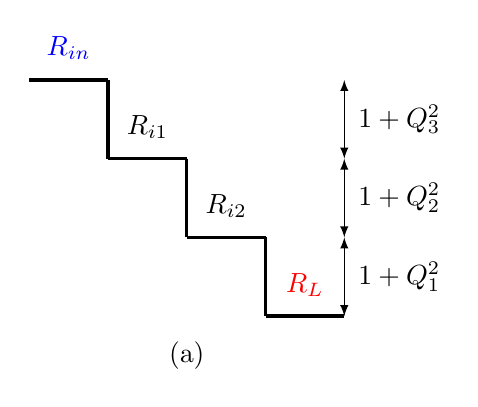
\begin{tikzpicture} 
    \draw[black, very thick] (-2,3) -- (-1,3);
    \draw[black, very thick] (-1,3) -- (-1,2);
    \draw[black, very thick] (-1,2) -- (0,2);
    \draw[black, very thick] (0,2) -- (0,1);
    \draw[black, very thick] (0,1) -- (1,1);
    \draw[black, very thick] (1,1) -- (1,0);
    \draw[black, very thick] (1,0) -- (2,0);

    \node[blue] at (-1.5,3.4) {$R_{in}$};  
    \node[red] at (1.5,0.4) {$R_{L}$}; 
    
    \node[black] at (-0.5,2.4) {$R_{i1}$};
    \node[black] at (0.5,1.4) {$R_{i2}$};
    
    \node[black] at (2.7,2.5) {$1+Q_3^2$}; 
    \node[black] at (2.7,1.5) {$1+Q_2^2$};
    \node[black] at (2.7,0.5) {$1+Q_1^2$};
    
    \draw[>=latex, <->] (2,3) -- (2,2);
    \draw[>=latex, <->] (2,2) -- (2,1);
    \draw[>=latex, <->] (2,1) -- (2,0);
    \node[black] at (0,-0.5) {(a)};
\end{tikzpicture}
};
\hspace{1cm}
\tikz \node [scale=0.7, inner sep=0] {
\begin{tikzpicture} [american]
    \draw[>=triangle 90, ->] (-5.5,0) -- (-4.5,0);
    \draw[>=triangle 90, ->] (6.5,0) -- (5.5,0);
    \draw[] (2,0.3) -- (2,0.8);
    \draw[>=triangle 90, ->] (-1,0.3) -- (-0.5,0.3);
    \draw[] (-1,0.3) -- (-1,0.8);
    \draw[>=triangle 90, ->] (2,0.3) -- (2.5,0.3);
    \node[black] at (2,1.2) {$R_{i1}$}; 
    \node[black] at (-1,1.2) {$R_{i2}$}; 
    \node[black] at (-5.9,0) {$R_{in}$}; 
    \node[black] at (6.9,0) {$R_L$}; 
    \node[black] at (0.5,-4) {(b)};
    \draw (2,0) to[L, l=$L_1$, *-*] (5,0)
    (2,0) to[C, l=$C_1$, *-] (2,-3) node[ground]{}
    (-1,0) to[L, l=$L_2$, *-*] (2,0)
    (-1,0) to[C, l=$C_2$, *-] (-1,-3) node[ground]{}
    (-4,0) to[L, l=$L_3$, *-*] (-1,0)
    (-4,0) to[C, l=$C_3$, *-] (-4,-3) node[ground]{}
    ;
\end{tikzpicture}
};

\caption{(a) Desired effect of impedance gain(b) Low-Q three sections network. Source: own.}
\label{graph:4} 
\end{figure}